\section{Camada de Adapta��o}

\begin{frame}
    \frametitle{C�lculo da Relev�ncia de uma P�gina}

    \begin{equation}
        \omega(o, d, g) = \frac{F_{odg}}{\sum_{t=1}^{n}F_{otg}}
        \label{eq:relevancia}
    \end{equation}

    \emph{onde:}

    \begin{itemize}
        \item $\omega$ � a relev�ncia daquela p�gina em rela��o �s outras;
        \item $n$ � o n�mero de p�ginas destino a partir daquela
        origem.
    \end{itemize}
\end{frame}

\begin{frame}
    \frametitle{Arquitetura do Modelo Proposto}

    \begin{figure}[htb]
        \begin{center}
            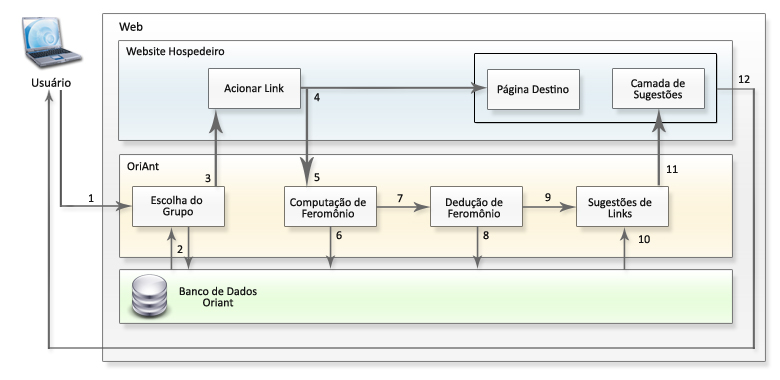
\includegraphics[width=\textwidth]{images/oriant/fig_geral.jpg}
            \label{fig:arquitetura}
            \caption{Arquitetura do modelo proposto}
        \end{center}
    \end{figure}

\end{frame}

\begin{frame}[t,allowframebreaks]
    \frametitle{Op��es para o usu�rio OriAnt}

    \begin{figure}[htb]
        \begin{center}
            
\includegraphics[width=10cm]{images/oriant/grupos.jpg}
            \label{fig:arquitetura}
            \caption{Grupo de interesses}
        \end{center}
    \end{figure}


    \begin{figure}[htb]
        \begin{center}
            
\includegraphics[width=10cm]{images/oriant/objetiva.jpg}
            \label{fig:arquitetura}
            \caption{Disposi��o objetiva}
        \end{center}
    \end{figure}

    \begin{figure}[htb]
        \begin{center}
            
\includegraphics[width=10cm]{images/oriant/orientada.jpg}
            \label{fig:arquitetura}
            \caption{Disposi��o orientada}
        \end{center}
    \end{figure}

    \begin{figure}[htb]
        \begin{center}
            
\includegraphics[width=10cm]{images/oriant/relacionada.jpg}
            \label{fig:arquitetura}
            \caption{Disposi��o relacionada}
        \end{center}
    \end{figure}

\end{frame}
